\documentclass[11pt]{article}
\usepackage{geometry,marginnote} % Pour passer au format A4
\geometry{hmargin=1cm, vmargin=1cm} % 

% Page et encodage
\usepackage[T1]{fontenc} % Use 8-bit encoding that has 256 glyphs
\usepackage[english,french]{babel} % Français et anglais
\usepackage[utf8]{inputenc} 

\usepackage{lmodern,numprint}
\setlength\parindent{0pt}

% Graphiques
\usepackage{graphicx,float,grffile,units}
\usepackage{tikz,pst-eucl,pst-plot,pstricks,pst-node,pstricks-add,pst-fun} 

% Maths et divers
\usepackage{amsmath,amsfonts,amssymb,amsthm,verbatim}
\usepackage{multicol,enumitem,url,eurosym,gensymb,tabularx}

\DeclareUnicodeCharacter{20AC}{\euro}



% Sections
\usepackage{sectsty} % Allows customizing section commands
\allsectionsfont{\centering \normalfont\scshape}

% Tête et pied de page
\usepackage{fancyhdr} \pagestyle{fancyplain} \fancyhead{} \fancyfoot{}

\renewcommand{\headrulewidth}{0pt} % Remove header underlines
\renewcommand{\footrulewidth}{0pt} % Remove footer underlines

\newcommand{\horrule}[1]{\rule{\linewidth}{#1}} % Create horizontal rule command with 1 argument of height

\newcommand{\Pointilles}[1][3]{%
  \multido{}{#1}{\makebox[\linewidth]{\dotfill}\\[\parskip]
}}

\newtheorem{Definition}{Définition}

\usepackage{siunitx}
\sisetup{
    detect-all,
    output-decimal-marker={,},
    group-minimum-digits = 3,
    group-separator={~},
    number-unit-separator={~},
    inter-unit-product={~}
}

\setlength{\columnseprule}{1pt}

\begin{document}

\textbf{Nom, Prénom :} \hspace{8cm} \textbf{Classe :} \hspace{3cm} \textbf{Date :}\\

\begin{center}
  \textit{Le salaire de l’école, ça vient plus tard, le salaire de l’école, ce sera un salaire justement !}  - \textbf{Pierrette Fleutiaux}
\end{center}

\subsection*{Cours : Statistiques :}

\Pointilles[5]

\subsection*{Exercices}

\textbf{EX1 - Calculer le min, max et étendue de chacune des séries.}

\begin{multicols}{3}

\begin{enumerate}
  \item[1a.] 5 ; 12 ; 14 ; 13 ; 15 ; 9 ; 12  \\ \Pointilles[5]
  \item[1b.] 4 ; -2  ; 30 ; -14 ; 0 ; 2,5 \\ \Pointilles[5]
  \item[1c.] $\dfrac{3}{2} ; \sqrt{2} ; \pi ; 3,14 ; 0 ; \dfrac{355}{113}; 6,01$ \\ \Pointilles[5]
\end{enumerate}

\end{multicols}

\textbf{EX2 - Calculer la moyennes de chacune des séries.}

\begin{multicols}{3}

  \begin{enumerate}
  \item[2a.] 5 ; 12 ; 14 ; 13 ; 15 ; 9 ; 12  \\ \Pointilles[3]
  \item[2b.] 4 ; -2  ; 30 ; -14 ; 0 ; 2,5 \\ \Pointilles[3]
  \item[2c.] $\dfrac{3}{2} ; \sqrt{2} ; \pi ; 3,14 ; 0 ; \dfrac{355}{113}; 6,01$  \\ \Pointilles[3]
\end{enumerate}

\end{multicols}

\textbf{EX3 - Calculer la moyenne de la série en tenant compte des coefficients.}

\begin{minipage}[t]{0.2\textwidth}
  \begin{itemize}[label={$\bullet$}]
    \item 12 coefficient 4
    \item 8 coefficient 2
    \item 10 coefficient 1
    \item 13 coefficient 3
    \item 6 coeffcient 3 
  \end{itemize}
\end{minipage}
\begin{minipage}[t]{0.8\textwidth}
  \Pointilles[6]
\end{minipage}

\textbf{EX4 - Calculer la médiane de chacune des séries.}

\begin{multicols}{3}

\begin{enumerate}
  \item[4a.] 5 ; 12 ; 14 ; 13 ; 15 ; 9 ; 12 \\ \Pointilles[5]
  \item[4b.] 4 ; -2  ; 30 ; -14 ; 0 ; 2,5 \\ \Pointilles[5]
  \item[4c.] $\dfrac{3}{2} ; \sqrt{2} ; \pi ; 3,14 ; 0 ; \dfrac{355}{113} ; 6,01$ \\ \Pointilles[5]
\end{enumerate}

\end{multicols}

\newpage

\textbf{EX5 - Tableur}

\begin{figure}[H]
  \centering
  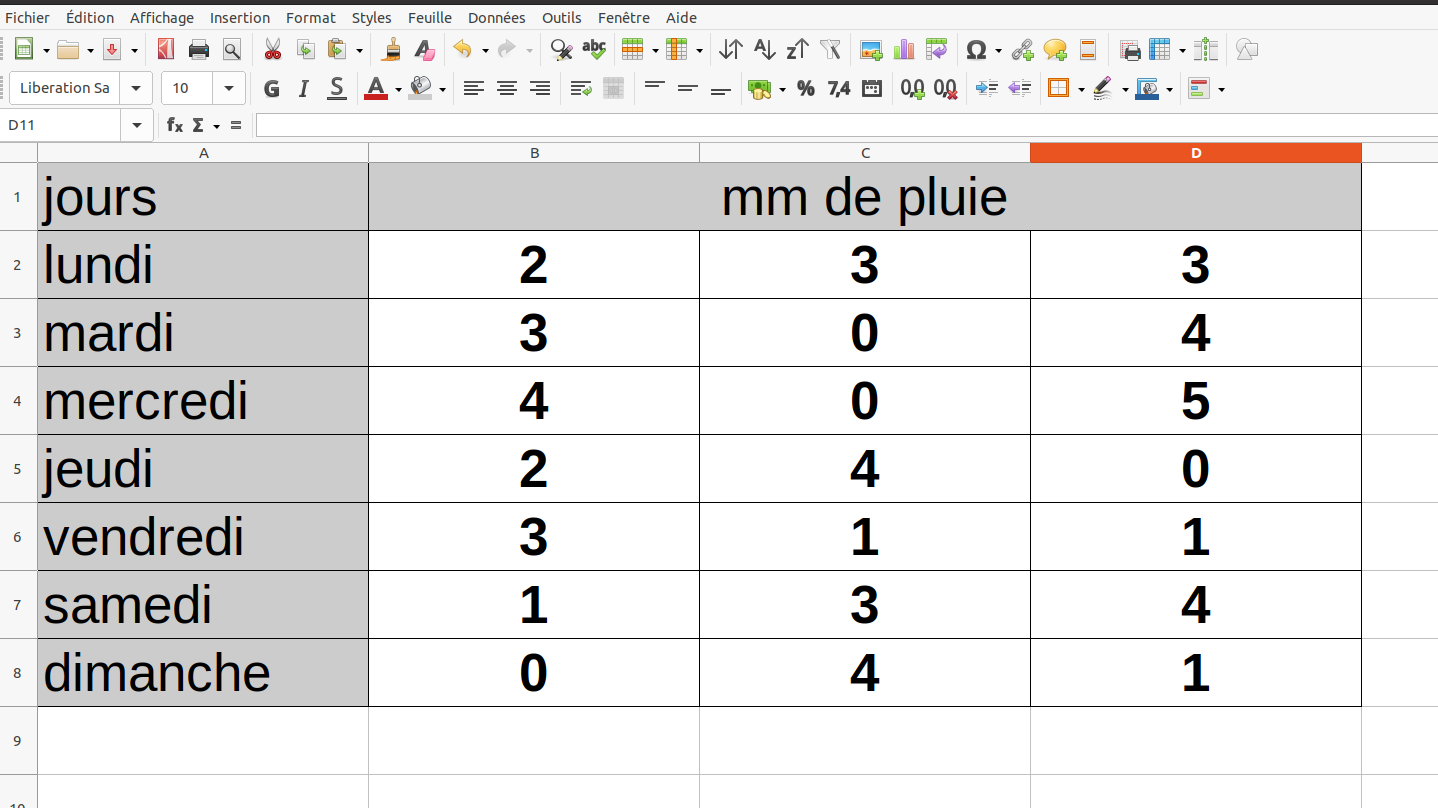
\includegraphics[width=0.5\linewidth]{4x8-statistiques/tab.png}
\end{figure}

\begin{enumerate}
  \item[5a.] Quel nombre est dans la case B4 ? \dotfill
  \item[5b.] Quelles cases ont pour valeur 4 ? \dotfill
  \item[5c.] Quelle formule écrire pour calculer la moyenne de tous les nombres de la colonne B ?  \\ \Pointilles[1]
\end{enumerate}

\subsubsection*{pb1}

Pendant le troisième trimestre, Henry a passé 4 évaluations. Il ne souvient que des trois dernières notes : 14 ; 12 et 8. Le professeur lui donne une moyenne de 10. 

\begin{enumerate}
  \item[pb1a.] Quelle est sa note lors de la première évaluation ? 
  \item[pb1b.] Il demande un DM coefficient 1 pour améliorer sa moyenne. Peut-il obtenir 13 de moyenne ?
\end{enumerate}

\Pointilles[8]

\subsubsection*{pb2}

Le basketteur Michael Jordan a participé à 29 matchs cette saison. Voilà son tableau des scores.

\begin{tabular}{|c|c|c|c|c|c|c|c|c|c|c|c|c|}
  \hline
  Nombre de points                         & 15 & 19 & 20 & 21 & 24 & 25 & 28 & 29 & 32 & 34 & 37 & 42 \\ \hline

  Nombre de match avec ce nombre de points & 2  & 3  & 1  & 4  &  3 & 2  & 6  & 1  & 3  & 1  & 2  & 1  \\ \hline
\end{tabular}

\begin{enumerate}
  \item[pb2a.] Calculer la moyenne des points par match.
  \item[pb2b.] Calculer la médiane des points par match.
\end{enumerate}

\Pointilles[8]

\end{document}

